\begin{frame}[fragile]{ProgressDialog en Android}
\textbf{¿Qué es ProgressDialog?}

\begin{itemize}
    \item Es un componente utilizado para mostrar un indicador de progreso al usuario.
    \item Se emplea comúnmente durante operaciones largas (carga de datos, procesos en segundo plano).
\end{itemize}


\textbf{Características:}
\begin{itemize}
    \item Puede mostrar un mensaje informativo.
    \item Puede ser cancelable o no por el usuario.
    \item Soporta estilos como barra de progreso o spinner.
\end{itemize}

\end{frame}


\begin{frame}[fragile]{Uso de AsyncTask para tareas en segundo plano}
\textbf{Clase: DownloadTask extends AsyncTask$<$String, Integer, List$<$String$>$$>$}

\begin{itemize}
    \item Permite ejecutar tareas en segundo plano sin bloquear la interfaz gráfica.
    \item Usa tres tipos genéricos:
    \begin{itemize}
        \item \textbf{String:} parámetros de entrada.
        \item \textbf{Integer:} progreso.
        \item \textbf{List$<$String$>$:} resultado final.
    \end{itemize}
\end{itemize}

\vspace{0.3cm}

\textbf{Fases del AsyncTask:}
\begin{itemize}
    \item \textbf{onPreExecute():} Inicializa variables y muestra el ProgressDialog.
    \item \textbf{doInBackground():} Ejecuta tareas en segundo plano, publica progreso y simula espera.
    \item \textbf{onProgressUpdate():} Actualiza la barra de progreso y mensaje.
    \item \textbf{onPostExecute():} Oculta el diálogo y muestra resultados en pantalla.
\end{itemize}



\end{frame}


\begin{frame}[fragile]
\frametitle{Demo 10: Progress Dialog y AsyncTask}
\begin{columns}
\column{0.80\linewidth}
Del Repositorio Github:
\begin{itemize}
\item Copiar el archivo \textit{MainActivity\_Demo10.java} (dentro del Folder códigosJAVA) al mismo directorio donde esta el MainActivity.java
\item Copiar el archivo \textit{activity\_main\_demo10.xml} (dentro del Folder Carpeta\_layout) al mismo directorio donde esta el activity\_main.xml
%\item Copiar los archivos \textit{cgup.jpg} y \textit{logo\_upv\_2019.png} localizados dentro de la folder \textit{Carpeta\_drawable} en el directorio \textit{res/drawable} del proyecto de AS.
\item Modificar en el archivo \textit{AndroidManifest.xml} la cadena \textit{.MainActivity\_Demo09} por \textit{.MainActivity\_Demo10}.
%\item Ir a la linea 22 de archivo del archivo \textit{MainActivity\_Demo09.java}, poner el cursos en la palabra (en Rojo) \textit{documentfile}, presionar la combinación ALT+ENTER, y seleccionar de la lista desplegable la opcion ``Add dependency on ....''. Esto quitará el error y hara los ajustes necesarios. 
\end{itemize}

%\begin{block}{Demo \#09}
%Un App que permite escribir el contenido de un EditText a un archivo y cargar el contenido de cualquier archivo en el EditText
%\end{block}


\column{0.20\linewidth}

\begin{center}
 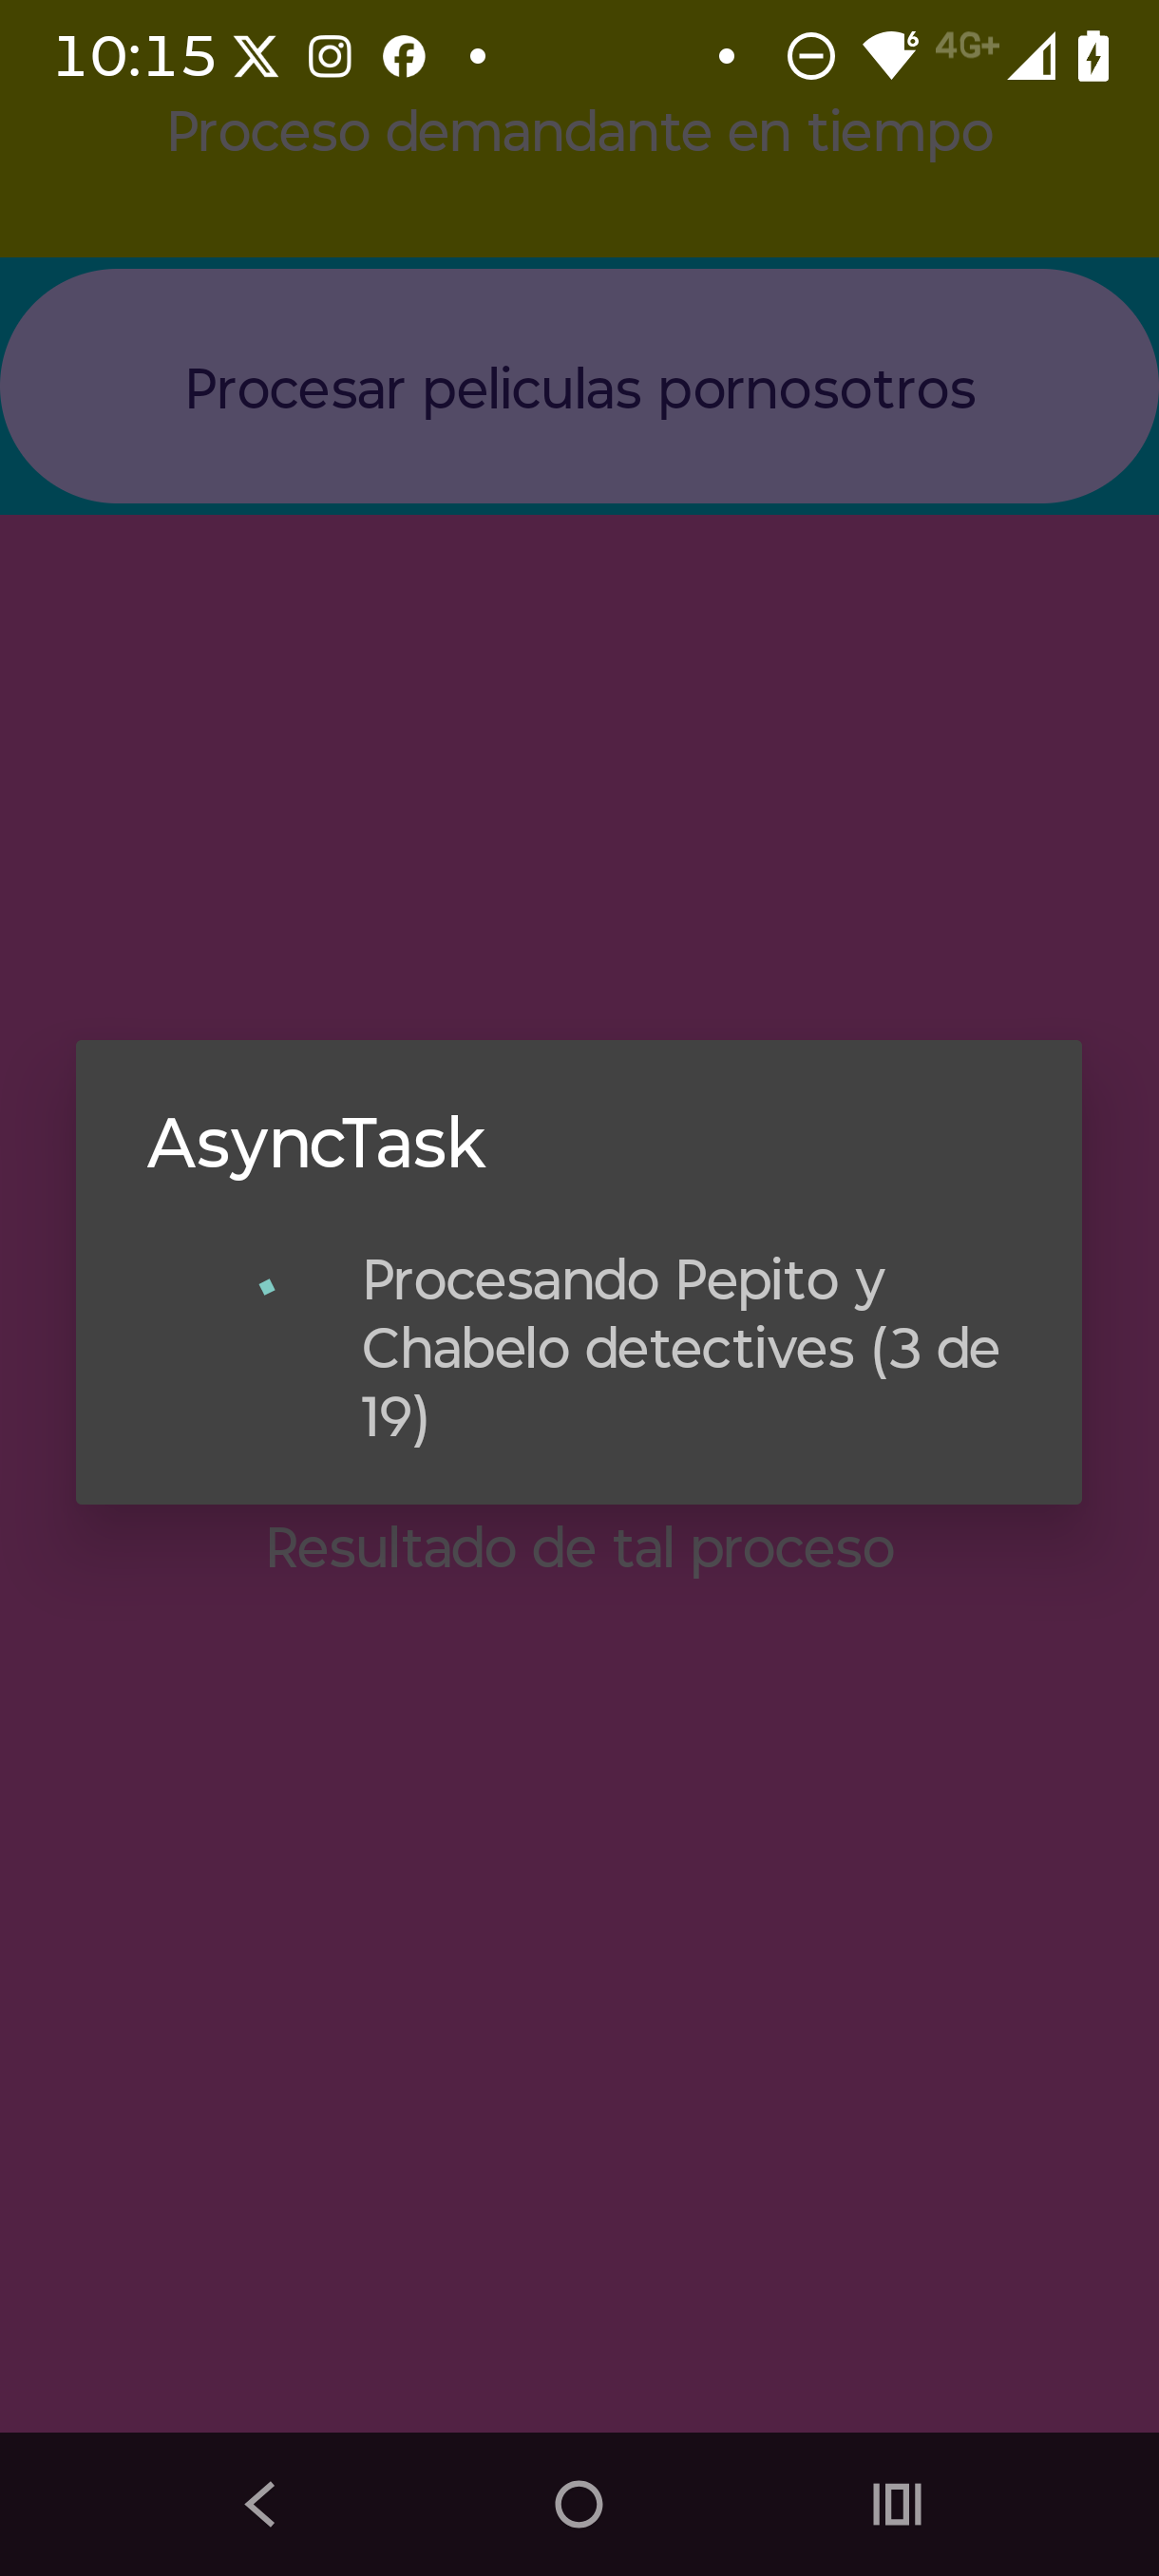
\includegraphics[width=0.98\textwidth]{02_TallerCBTis/figs/Demo10}
\end{center}

\end{columns}

\end{frame}

